%%%%%%%%%%%%%%%%%%%%%%% file template.tex %%%%%%%%%%%%%%%%%%%%%%%%%
%
% This is a general template file for the LaTeX package SVJour3
% for Springer journals.          Springer Heidelberg 2010/09/16
%
% Copy it to a new file with a new name and use it as the basis
% for your article. Delete % signs as needed.
%
% This template includes a few options for different layouts and
% content for various journals. Please consult a previous issue of
% your journal as needed.
%
%%%%%%%%%%%%%%%%%%%%%%%%%%%%%%%%%%%%%%%%%%%%%%%%%%%%%%%%%%%%%%%%%%%
%
% First comes an example EPS file -- just ignore it and
% proceed on the \documentclass line
% your LaTeX will extract the file if required
%\begin{filecontents*}{example.eps}
%!PS-Adobe-3.0 EPSF-3.0
%%BoundingBox: 19 19 221 221
%%CreationDate: Mon Sep 29 1997
%%Creator: programmed by hand (JK)
%%EndComments
%gsave
%newpath
%  20 20 moveto
%  20 220 lineto
%  220 220 lineto
%  220 20 lineto
%closepath
%2 setlinewidth
%gsave
%  .4 setgray fill
%grestore
%stroke
%grestore
%\end{filecontents*}
%
\RequirePackage{fix-cm}
%
%\documentclass{svjour3}                     % onecolumn (standard format)
%\documentclass[smallcondensed]{svjour3}     % onecolumn (ditto)
\documentclass[smallextended]{svjour3}
\usepackage{amsmath}
% onecolumn (second format)
%\documentclass[twocolumn]{svjour3}          % twocolumn
%
\smartqed  % flush right qed marks, e.g. at end of proof
%
\usepackage{graphicx}
\usepackage{bbm}
%\usepackage{epstopdf}
\usepackage[outdir=./figure/]{epstopdf}
%\usepackage[outdir=./]{epstopdf}
%\graphicspath{{./figure/}}
%
% \usepackage{mathptmx}      % use Times fonts if available on your TeX system
%
% insert here the call for the packages your document requires
%\usepackage{latexsym}
% etc.
%
% please place your own definitions here and don't use \def but
% \newcommand{}{}
%
% Insert the name of "your journal" with
% \journalname{myjournal}
%


\usepackage{color}
\newcommand{\rd}[1]{{\color{red}{#1}}}


\begin{document}

%\title{Analysis of disk crack pattern using peridynamics with machine learning}
\title{Analysis of crack patterns using peridynamic simulations and deep neural networks}
%\subtitle{Do you have a subtitle?\\ If so, write it here}

%\titlerunning{Short form of title}        % if too long for running head

\author{Moonseop Kim \and Nick Winovich \and Guang Lin \and Wontae Jeong}

%\authorrunning{Short form of author list} % if too long for running head

\institute{*Corresponding author at: Department of Mechanical Engineering, Purdue University,
West Lafayette, IN 47906-2045, Tel.: +1 765 494 1965\\
\email{guanglin@purdue.edu (Guang Lin), kim2122@purdue.edu (Moonseop Kim), nwinovic@purdue.edu (Nick Winovich),        
}
}
\date{Received: date / Accepted: date}
% The correct dates will be entered by the editor


\maketitle

\begin{abstract}
  %%
  In this work, we introduce convolutional neural networks designed to predict and analyze damage patterns on a disk resulting from molecular dynamics (MD) collision simulations.
  %%
  The simulations under consideration are specifically designed to produce cracks on the disk and, accordingly, numerical methods which require partial derivative information, such as finite element analysis, are not applicable.
  %%
  These simulations can, however, be carried out using peridynamics, a nonlocal extension of classical continuum mechanics
  based on integral equations which overcome the difficulties in modeling deformation discontinuities.
  %%
  Though this  nonlocal extension provides a highly accurate model for the MD simulations,
  the computational complexity and corresponding run times increase greatly as the simulations grow larger.
  %%
  We propose the use of  neural network approximations to complement peridynamic simulations
  by providing quick estimates which maintain much of the accuracy of the full simulations
  while reducing simulation times by a factor of $1,500$.
  %simulation times by a factor of $1,500$ while maintining much of the accuracy of the full simulations.
  %%
  We propose two distinct convolutional neural networks: one trained to perform the {\emph{forward problem}} of predicting the damage pattern on a disk provided the location of a colliding object's impact, and another trained to solve the {\emph{inverse problem}} of identifying the collision location, angle, velocity, and size given the resulting damage pattern.

  %Using the advantage of crack analysis of peridynamics, this study produced data using peridynamics for the material of crack pattern.
  %%
  %Based on molecular dynamics (MD) simulations, machine learning and peridynamics are applied to prediction of disk damage patterns for the forward problem and conversely, in inverse problem, damage pattern of the disk is used to predict the size, angle and velocity of the indenter.
  %%
  %Peridynamics is the nonlocal extension of classical continuum mechanics and same as MD model.
  %%
  %Especially, FEM is based on the partial differential equations.
  %%
  %However, partial derivatives do not exist on the crack and damage surfaces.
  %%
  %To complement this problem, peridynamics was used which is based on the integral equations and overcome deficiencies in the modeling of deformation discontinuities.
  %%
  %Using the advantage of crack analysis of peridynamics, this study produced data using peridynamics for the material of crack pattern.
  %%
  %In this study, the forward problem (i), if we have images of damage and crack, crack patterns are predicted using trained data compared to true solutions which are hit by changing the $x$ and $z$ hitting coordinates on the disk.
  %%
  %The inverse problem (ii), if we have images of damage and crack, the corresponding hitting location, the velocity of indenter, the angle of indenter and the size of indenter are predicted using trained data.
  %%
  \keywords{Peridynamics \and Crack patterns \and Molecular dynamic simulation \and Machine learning \and Convolutional neural network}
  % \PACS{PACS code1 \and PACS code2 \and more}
  % \subclass{MSC code1 \and MSC code2 \and more}
\end{abstract}

\section{Introduction}
\label{sec:1}
%Many products in everyday life are damaged by external shocks or user's mistakes, and cracks are formed. In the Department Of Energy (DOE), it is often the case that blades of thermoelectric power plant and wind power plant are damaged by rotation, temperature effects, and external wind influences. In the reactor of the nuclear power plant, cracks are occurred due to heat generated during nuclear fission. This can lead to not only high maintenance costs but also a national disaster. So far, research on cracking has been going on in various perspectives for several decades.
%%
%Representatively, various types of structures and material behaviors have been studied through the finite element analysis (FEM). However, there are inherent errors in the study through the FEM. In the FEM, only the approximate solution can be obtained. Also, the results of analysis tend to depend on the mesh, and the mistakes by the researchers can be fatal to derive the results.
%%
The finite element method (FEM) is
founded on the basis of partial differential equations;
since partial derivatives may not always be defined on surfaces with cracks, however,
the FEM model cannot be used to obtain accurate results for crack pattern analysis.
%%
%Therefore, i
In order to compensate for these drawbacks, we conducted a crack pattern study using peridynamics.
%%
The peridynamics theory of solid mechanics was first introduced by S. Silling \cite{Ref1,Ref2,Ref3,Ref4}.
%%
This theory is a nonlocal extension of classical continuum mechanics and provides an alternative to continuum mechanics for more accurate crack studies.
%%
This model is based on integral equations, which can be applied directly to cracks with the advantage of not requiring to compute partial derivatives.
%%
Therefore, peridynamics is very suitable for the study of surface discontinuities such as cracks.
%%
Peridynamics can be of particular use in understanding the damage in membranes and nanofiber \cite{Ref5}, composites and brittle materials \cite{Ref6}, brazed single-lap joints \cite{Ref7}, fuel pellet \cite{Ref8} and biomembranes \cite{Ref9}.
%%
Peridynamics can be applied not only to damage studies, but also to technologically important areas such as prediction of viscoelastic materials \cite{Ref10}, piezo-resistive response of carbon nanotube nanocomposites \cite{Ref11}, phase transformation in zirconium dioxide \cite{Ref12}, shock and vibration \cite{Ref13}, and indentation of thin copper film \cite{Ref14}.
%%


Though the peridynamics framework has proven to be a powerful and widely applicable tool, the computational demand can become burdensome very quickly as the scales of the simulations are increased.
%%
In order to decrease the computation time required to run these simulations while maintaining a high level of accuracy, we propose a machine learning approach which utilizes recent design and hardware advances that have greatly improved the performance of artificial neural networks (ANNs).
%%
Recently, convolutional neural networks (CNNs) have been shown to provide an excellent light-weight alternative to traditional fully-connected networks, and are particularly well-suited for applications on highly structured data, which is characteristic of the systems considered in peridynamics.
%%
These networks have the advantage of being trainable in advance, learning from a dataset generated by a highly accurate model such as peridynamics and encoding an approximation of the model into a concise, neural network representation; this approximate model can then be used after the training procedure to produce near instantaneous results.
%%
By combining the accuracy of the peridynamics model with the computational speed of modern neural networks, we show that complex MD simulations can be accurately performed using just a fraction of the computation time required by traditional approaches.

\section{The peridynamics model}
\label{sec:2}

% For one-column wide figures use
\begin{figure}
% Use the relevant command to insert your figure file.
% For example, with the graphicx package use
  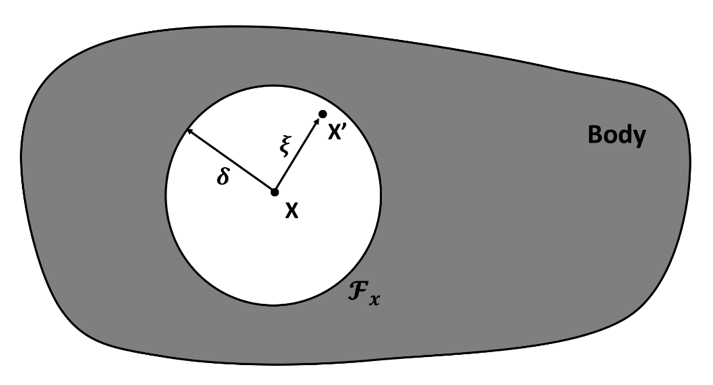
\includegraphics{figure/body.eps}
% figure caption is below the figure
\caption{The composition of peridynamics model.}
\label{fig:1}       % Give a unique label
\end{figure}

Peridynamics is the non-local extension of classical continuum mechanics \cite{Ref15}. The model structure of peridynamics is essentially the same as an MD model, and simulations can be conducted in LAMMPS~\cite{Ref16} using the
standard SI units (m, kg, sec etc.).
%{\rd{and in LAMMPS, SI units (m, kg, sec etc.) can be used for simulations}}.
%Compared with FEM (Finite Element Method), FEM can only acquire approximate solutions and the user's mistake in obtaining a solution can be incredibly deadly, and the results can vary depending on how the mesh is set.
%%
%Finally,
The finite element method (FEM) approach is based on partial differential equations, but these partial derivatives do not exist on the crack surfaces.
%%
However, a peridynamics model can be used to overcome this difficulty.
%%
The peridynamics model formulation is based on integral equations.
%%
In the analysis of damage and cracks, the integral equations of the peridynamics theory can be applied directly, since it does not require partial derivatives.
%%
Accordingly, it overcomes deficiencies in the modeling of deformation discontinuities.
%%
Next, let us look at the governing equations of the peridynamics model \cite{Ref2,Ref3,Ref4}.
%%
%Fig. 1 is plotted to represent the composition of the peridynamics model.
Fig.~\ref{fig:1} gives an overview of the composition of the peridynamics model.
%%
For each point $x$ in the reference configuration, we define the family $\mathcal{F}_x$ to consist of all points $x'$ in the body which are within the horizon $\delta$ boundary of $x$.
In peridynamics theory, all points in a given family $\mathcal{F}_x$ are interconnected by bonds; that is, each point has connectivity to all points in the horizon $\delta$ of itself as well as nearby neighbors.
%%
%As illustrated in Fig.~\ref{fig:1}, $\mathcal{F}_x$ (the family of $x$) is contained in the body, and  $x$ and ${x'}$ represent arbitrary points inside of the body. %%
%{\rd{$x$ and ${x'}$ are the points given in the reference configuration}}.
%%
%$u(x,t)$ and $y(x,t)$ represent the displacement and position of the point $x$ at time $t$, respectively.
%%
%In peridynamics theory, all points, including $x$ and ${x'}$ in the horizon $\delta$ boundary, are interconnected by bonds.
%%
%That is, each point {\rd{has connectivity to all points in horizon $\delta$ as well as nearby neighbors}}.
%%
Thus peridynamics is a non-local extension of the classical continuum mechanics, with the horizon parameter $\delta$ determining the extent of the non-local interactions modeled. 
%%
%{\rd{The integral equation is accustomed to calculate the current point forces per unit volume.}}
%%
Since spatial differentiation is not used in peridynamics, it is useful for analyzing discontinuous media and discrete particles such as cracks or damage.
%%
%$u(x,t)$ and $y(x,t)$ represent the displacement and position of the point $x$ at time $t$, respectively.
Denoting the displacement and position of the point $x$ at time $t$ by $u(x,t)$ and $y(x,t)$, respectively,
the peridynamic equation of motion is given by:
%eq1 
\begin{equation}
\rho(x) \, \ddot{u}(x,t) \, \, = \, \, \int_{\mathcal{F}_x} \omega\left(u(x',t)-u(x,t),x'-x\right) \, \, dV_{x'} \, \, + \, \, b(x,t), \quad t\geq0
\end{equation}

\noindent where $\rho(x)$ is the density in the reference configuration, $F_x$ is the family of $x$ in the horizon $\delta$, $b$ indicates the external force per unit volume and $u$ represent the displacement of the point $x$ at time $t$. $\omega$ is the pairwise bond force density that includes all of the information related to $x$ and ${x'}$.
%%
%Next, the relative position vector which is time-independent and displacement vector which is time-dependent of two bonded points $x$ and ${x'}$ are defined by $\zeta$ = ${x'}$ - $x$ and $\eta$ = $u$(${x'}$,$t$) - $u$($x$,$t$), respectively.
Next, the time-independent relative position vector and time-dependent displacement vector of two bonded points $x$ and ${x'}$ are defined by $\zeta$ = ${x'}$ - $x$ and $\eta$ = $u$(${x'}$,$t$) - $u$($x$,$t$), respectively.
$\zeta$ + $\eta$ represents the current relative position vector between the particles. The pairwise bond force density $\omega$ have the following properties: 
%eq2
\begin{equation}
\omega(-\eta,-\zeta)= -\omega(\eta, \zeta),\quad(\zeta + \eta)\times\omega(\eta, \zeta)=0 \quad\forall\eta,\zeta
\end{equation}




\noindent where $\omega(-\eta,-\zeta)= -\omega(\eta, \zeta)$ represents the conservation of linear momentum, and $(\zeta + \eta)\times\omega(\eta, \zeta)=0$ indicates the conservation of angular momentum. This implies that the force vector between $x$ and ${x'}$ is parallel to their current relative position vector. In this study, the crack pattern generated by impact of an indenter on a disk is used as input data of a machine learning algorithm. More specifically, a Prototype Microelastic Brittle (PMB) model \cite{Ref4} was used for the constitutive model to obtain a more precise and complex crack pattern. The governing equations are given as: 

%eq3
\begin{equation}
s=\frac{|\zeta+\eta|-|\zeta|}{|\zeta|}=\frac{y-|\zeta|}{|\zeta|}
\end{equation}

\noindent where $f$ is the scalar valued bond force defined in relation to bond stretch $s$. The best way {\rf{to apply failure}} to the constitutive model is to allow the bonds to break when they exceed a predefined limit. If the bond is broken, the tensile strength cannot be restored. The PMB model is defined as follows:
%eq4
\begin{equation}
f(y(t),\zeta)=g(s(t,\zeta))\mu(t,\zeta)
\end{equation}
%eq5
\begin{equation}
g(s)=cs \quad\forall s
\end{equation}

%eq6
\begin{equation}
  \mu(t,\zeta) = \left \{
  \begin{aligned}
    &1, && \textrm{if} \quad s(t',\zeta)<s_0 \quad \textrm{for all} \quad 0 \leq t' \leq t\\
    &0, && otherwise
  \end{aligned} \right.
\end{equation}


\noindent where $f$ is composed of the products of the $g$ and $\mu$ functions. $g$ is the linear scalar-valued function which is composed of the spring constant $c$ and bond stretch $s$. $\mu$ is a history-dependent scalar-valued function and has a value of 1 and 0 depending on the following condition: if the bond stretch is less than the critical bond stretch $s_0$, it has a value of 1, otherwise it has a value of 0. The spring constant $c$ and the critical bond stretch $s_0$ mentioned above are described in detail below.
%Text with citations \cite{RefB} and \cite{RefJ}.
%\subsection{Subsection title}
%\label{sec:2}
%as required. Don't forget to give each section
%and subsection a unique label (see Sect.~\ref{sec:1}).
%\paragraph{Paragraph headings} Use paragraph headings as needed.

%eq7
 \begin{equation}
\frac{18k}{\pi\delta^4}
\end{equation}

%eq8
 \begin{equation}
G_0=\frac{\pi cs_0^2\delta^5}{10} 
\end{equation}

%eq9
 \begin{equation}
s_0=\sqrt{\frac{10G_0}{\pi c\delta^5}}=\sqrt{\frac{5G_0}{9 k\delta}}
\end{equation}

 \noindent Here $k$ is the bulk modulus of the material and $G_0$ is the shear modulus.%, work required to crack all bonds in a unit fracture area.
 As seen from the equations above, the spring constant and the critical bond stretch are composed of the bulk modulus of the material $k$ and the chosen horizon boundary $\delta$.
 %%
 However, in the case of brittle materials such as glass, the assumption that the critical bond stretch $s_0$ is constant is an oversimplification.  These materials can be better modeled by defining $s_0$ in terms of the minimum stretch $s_{min}$ between all bonds connected to a given point $x_0$ via:

 \begin{equation}
s_0=s_{00}-\alpha s_{min}(t), \quad s_{min}(t)  \, = \, \min_\zeta \, {\frac{y(x_0,t)-|\zeta|}{|\zeta|}}
\end{equation}

 \noindent %where $s_{min}$ is the current minimum stretch in the group of all bonds linked to a given point.
 where $s_{00}$ and $\alpha$ are material-dependent constants with $\alpha$ generally set to about 1/4~\cite{Ref4}. 

\section{Preparation of MD data using the peridynamics model }
\label{sec:3}

In this study, crack pattern data was generated using the peridynamics model implemented in LAMMPS \cite{Ref16}, an MD simulation tool.
%%
A spherical indenter is designed to impact a thin cylindrical disk in the direction perpendicular to the face of the disk.
%%
For both the forward and inverse problems, the impact location of the indenter has varied across the face of the disk.
%{\rd{A spherical indenter impacted the disk by dropping the spherical indenter in the direction perpendicular to the disk, it means from the ${+y}$ axis to disk and varying the $x$ and $z$ coordinates of the indenter to impact whole parts of the disk.}}
%%
For the forward problem, the radius and velocity of the indenter were fixed at 0.002m and 100m/s, respectively.
%%
For the inverse problem, the indenter varied between two radius sizes, 0.007m and 0.008m, and two velocites, 100m/s and 100.1m/s.
In addition, the impact angle of the indenter has been simulated at both $0^{\circ}$ and $45^{\circ}$.
%The radius of the indenter are 0.007m and 0.008m for the inverse problem
%and the velocity are 100m/s and 100.1m/s,
%however, for the forward problem, the radius of the indenter and velocity are fixed by 0.0020m and 100m/s respectively.
%%
%The radius of the cylindrical disk is 0.037m, the thickness is 0.0025m and this disk contains 103,110 particles.
The cylindrical disk impacted by the indenter has been assigned a radius of 0.037m, thickness of 0.0025m, and consists of 103,110 particles.
%%
Each particle $i$ has volume fraction $V_i$=1.25 \times 10$^{-10}$m$^3$, and the density of the disk material is $\rho$=2200kg/m$^3$.
%%
The `peri/pmb' peridynamic pair style was selected for the simulations conducted using LAMMPS.
%%
%{\rd{Pair constants are $c$, horizon, $s_{00}$ and $\alpha$ in order of 1.6863e22, 0.0015001, 0.0005, 0.25 respectively.}}
The pair constants for the simulations have been specified as follows: $c=1.6863\mathrm{e}22$, horizon $\delta$ equal to $0.0015001$, $s_{00}= 0.0005$, and $\alpha = 0.25$.
%%
$c$ is the spring constant for peridynamic bonds, the horizon $\delta$ is a cutoff distance for non-local interactions,
%%
and the constants $s_{00}$ and $\alpha$ correspond to material-dependent parameters for the critical bond stretch.
%%
The LAMMPS MD simulation tool (PDLAMMPS) \cite{Ref17,Ref18} is used to obtain the crack pattern data generated by the indenter using peridynamics simulations,
%%
with the hitting location, velocity, radius, and impact angle of the indenter varied as described above.
%{\rd{and obtain the specific data by changing the variable using for loops to adjust the velocity and radius of the indenter and the hitting point of the disk.}}
%%
SI units are used and the boundary conditions are ``shrink-wrapped'' to ensure all atoms are retained in the computation.
%%
The particle volume used has been set to a simple cubic lattice with lattice constant 0.001m.
%%
A cylinder disk (target) with radius 0.037m and thickness 0.0025 m is initialized.
%%
The initial velocity of all particles is set to zero, and the hitting location, velocity, impact angle, and radius of the indenter are then specified.
%%
%In addition, for the inverse problem, the damage is given to the whole parts of the target, but in the forward problem, peridynamics proved to be inaccurate in the boundary part, and data is obtained by only damaging 1/5 size around the center of the target.
For the inverse problem, the indenter hit locations are varied throughout the whole of the target disk;
in the forward problem, however, only the inner third of the disk has been targeted in order to avoid inaccuracies in the peridynamics simulation caused by the disk's boundary.
%%
Once the parameters have been specified, the simulation is carried out for 2000 time steps, and the resulting crack pattern image along with the indenter parameters are saved for use in the neural network training procedure.
%%
%{\rd{Finally, a dump command is used to obtain the crack pattern image, and 2000 time-steps of running simulation to get the data are used, and we set it to 2000 time-steps in dump command as well.}}
%%
%{\rd{The reason for this is that the image we want for the prediction in the next step is the initial image and the final image due to the same as the meaning of 2000 in the dump command is to store the $x$,$z$ coordinates of the atoms at the initial target and 2000 time-steps of the target. }}

\begin{figure}[h]
\begin{subfigure}
  %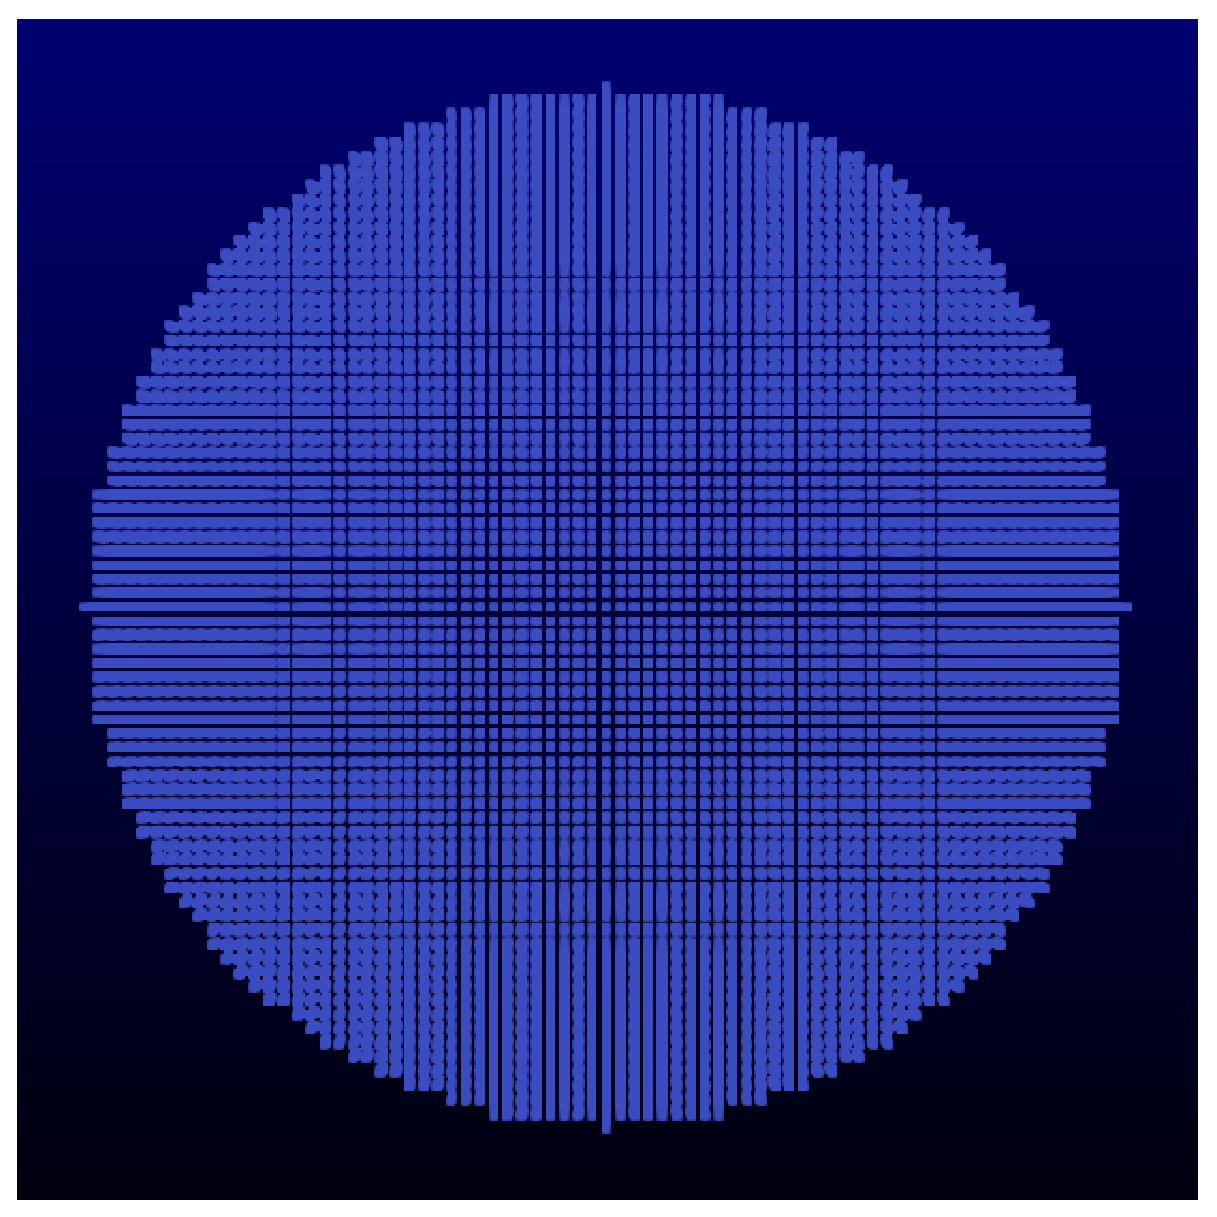
\includegraphics[width=5.8cm,height=5.8cm]{figure/initialdisk.eps}
  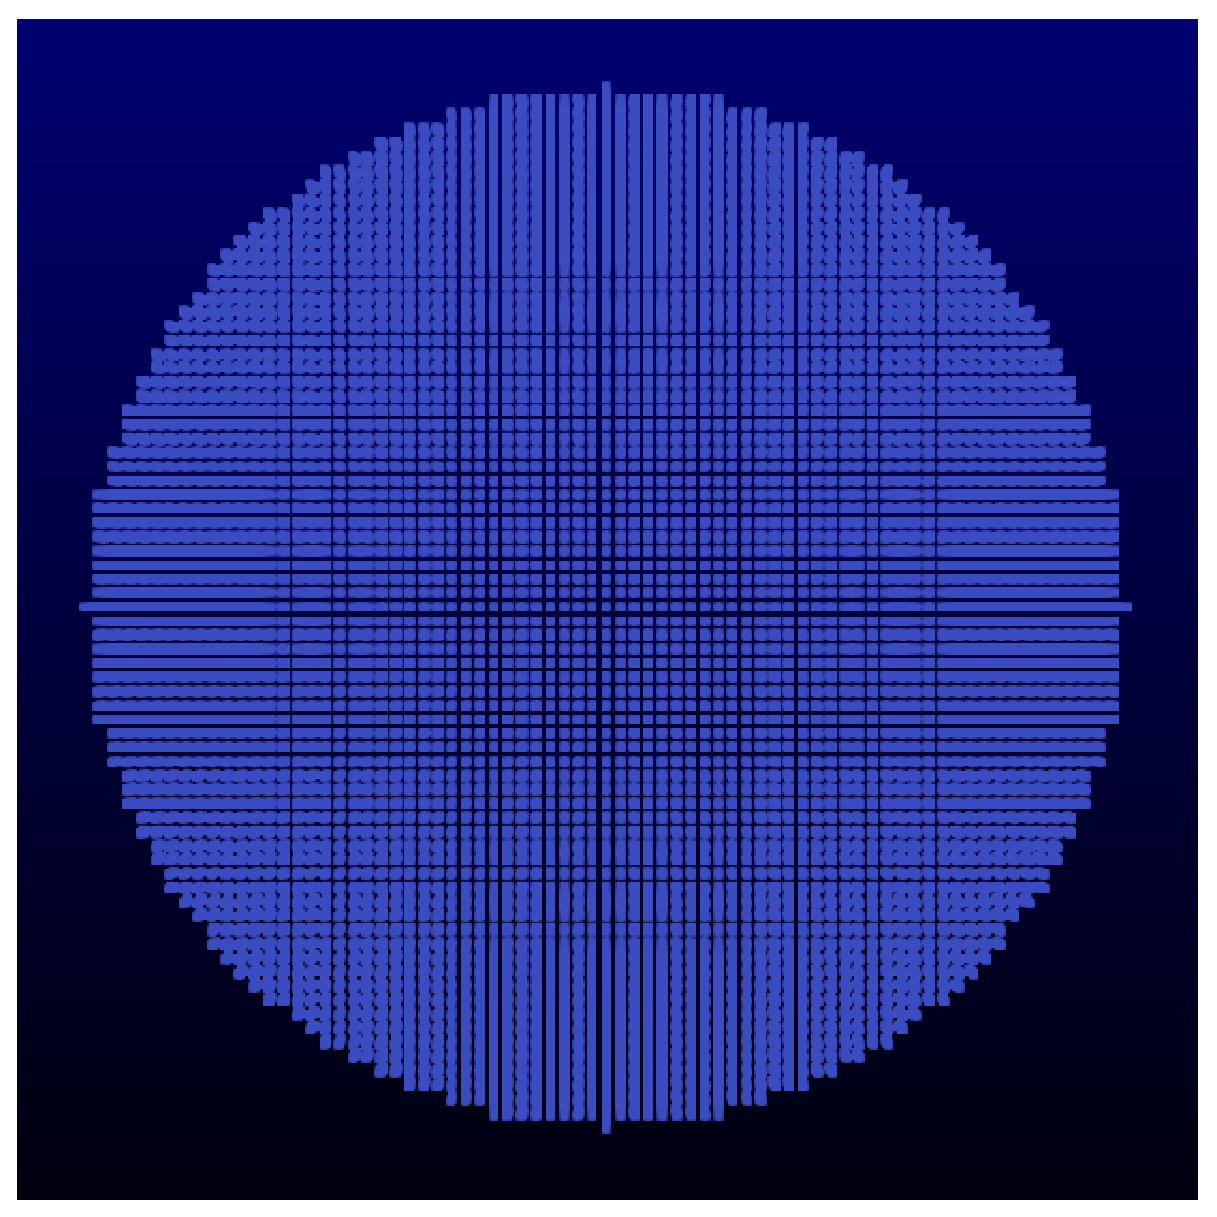
\includegraphics[height=5.8cm]{figure/initialdisk.eps}
\label{initial}
\end{subfigure}
\begin{subfigure}
  %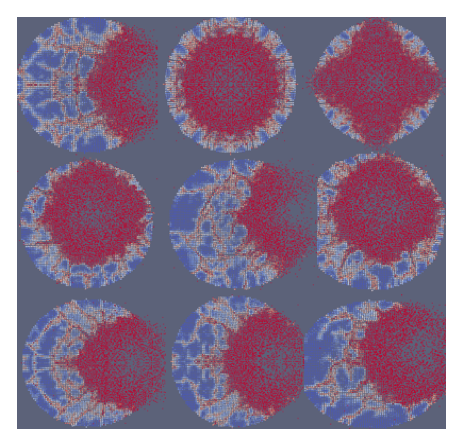
\includegraphics[width=5.8cm,height=5.8cm]{figure/damage.eps}
  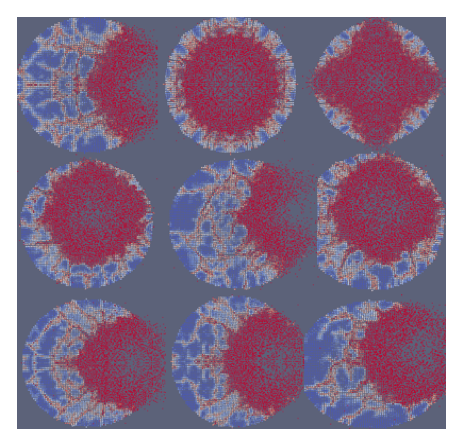
\includegraphics[height=5.8cm]{figure/damage.eps}
\label{damage}
\end{subfigure}
\caption{The initial appearance of the disk (Left) and the data results after hitting the indenter onto the disk (Right).}
\label{fig:2}
\end{figure}

%%Using the LAMMPS setup described above, we can see the results obtained by simulation using LAMMPS tool in Fig. 2.
A collection of LAMMPS simulation results using the setup described above are illustrated in Fig.~\ref{fig:2}.
%%
The dump file after running the MD simulation is changed to the EnSight data format with the pizza.py toolkit \cite{Ref19} and Paraview is used for data visualization as shown in Fig.~\ref{fig:2} \cite{Ref20}.
%%
The figure to the left shows the initial model of the target disk, and the figure to the right shows the same disk at the end of the simulation.
%%
The high level of symmetry in the peridynamics solutions is a consequence of using a perfect lattice and perfectly spherical indenter. 
%%
The use of asymmetric crack patterns could provide better data for real world applications,
but in this work we have focused primarily on the symmetric case in order to simplify the peridynamics modeling setup.
%focused primarily on crack patterns with symmetry, However, as the position of the hitting point change, various crack patterns can be confirmed, so that the data for machine learning is sufficient.
%4
\section{Results and Discussion}
\label{sec:4}


\begin{figure}
  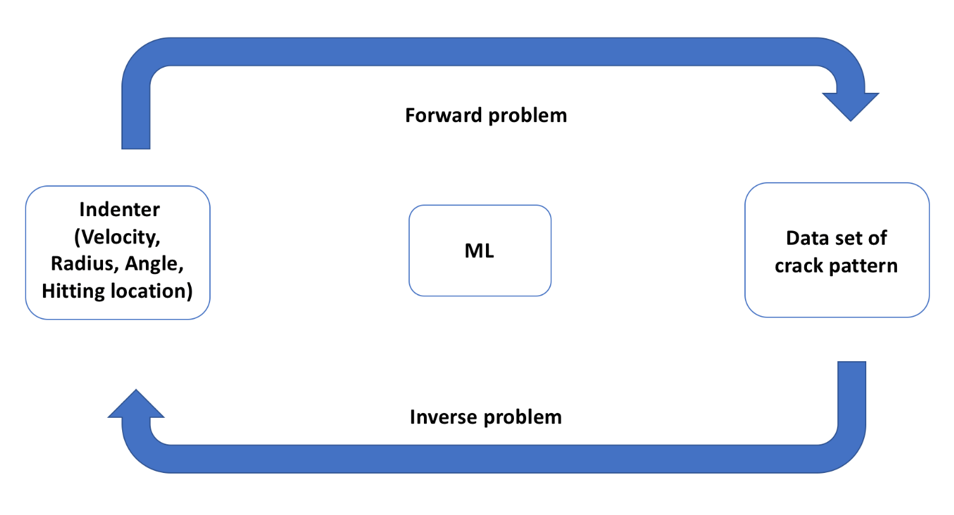
\includegraphics[width=12cm, height=7cm]{figure/diagram.eps}

\caption{Diagram of forward problem and inverse problem using machine learning algorithm.}
\label{fig:3}       
\end{figure}

In this study, data obtained from peridynamics simulations is used to predict solutions for forward and inverse problems using a machine learning algorithm as illustrated in the diagram presented in Fig.~\ref{fig:3}.
%%
For the forward problem, the crack patterns of the target disk are predicted based on the known hitting location of the indenter.
%%
Conversely, for the inverse problem, crack patterns are used to predict the velocity, radius, hitting angle, and hitting location of the indenter.

%4.1
\subsection{Dataset creation for the forward problem}
\label{forward_data}

The dataset for the forward problem has been created using the LAMPPS peridynamics package.  Simulations corresponding to  25,250 indenter hit locations were carried out to construct the final dataset.  To avoid the introduction of potentially unrealistic artifacts in the dataset due to inaccuracies of the peridynamics model near the boundary, the selected hitting locations have been restricted to the inner $1/3$ of the target disk.

In order to successfully train the network for the forward problem, it was necessary to design a loss function which converted the raw LAMMPS damage data into a format which is compatible with the deep learning framework and array/tensor-based format of the TensorFlow network implementation.  This conversion was performed most naturally by bucketizing the atoms into a uniform grid of resolution $64 \times 64$.  The average damage of the atoms contained in each bucket/bin of the grid was calculated and used to create the target outputs for the network.  It was also necessary to account for atoms which had been substantially dislocated by a direct impact with the indenter and had left some bins at the disk's interior empty.  These interior bins were assigned a full damage value of $1.0$ to indicate that the atom which had originally occupied the space was displaced by the indenter.  This was achieved by storing a copy of the LAMMPS data before the indenter strikes to serve as a template which indicates where the atom damages should be calculated.


\subsubsection{Network structure for the forward problem}
\label{forward_network}

To accomplish this task, we propose the use of a deep neural network which consists of several dense, fully-connected network layers followed by a sequence of transpose convolutional layers.  In this framework, the input coordinates are first processed by the initial dense network layers to construct features which are reshaped into a collection of coarse $8 \times 8$ resolution features.  These coarse features are then passed to the transpose convolutional layers to be upsampled into a single, higher resolution $64 \times 64$ damage pattern prediction.  The precise network structure used is shown in figure \ref{fig:forward}.  This network was implemented using the TensorFlow software library and written in Python.

\begin{figure}
  \centering
  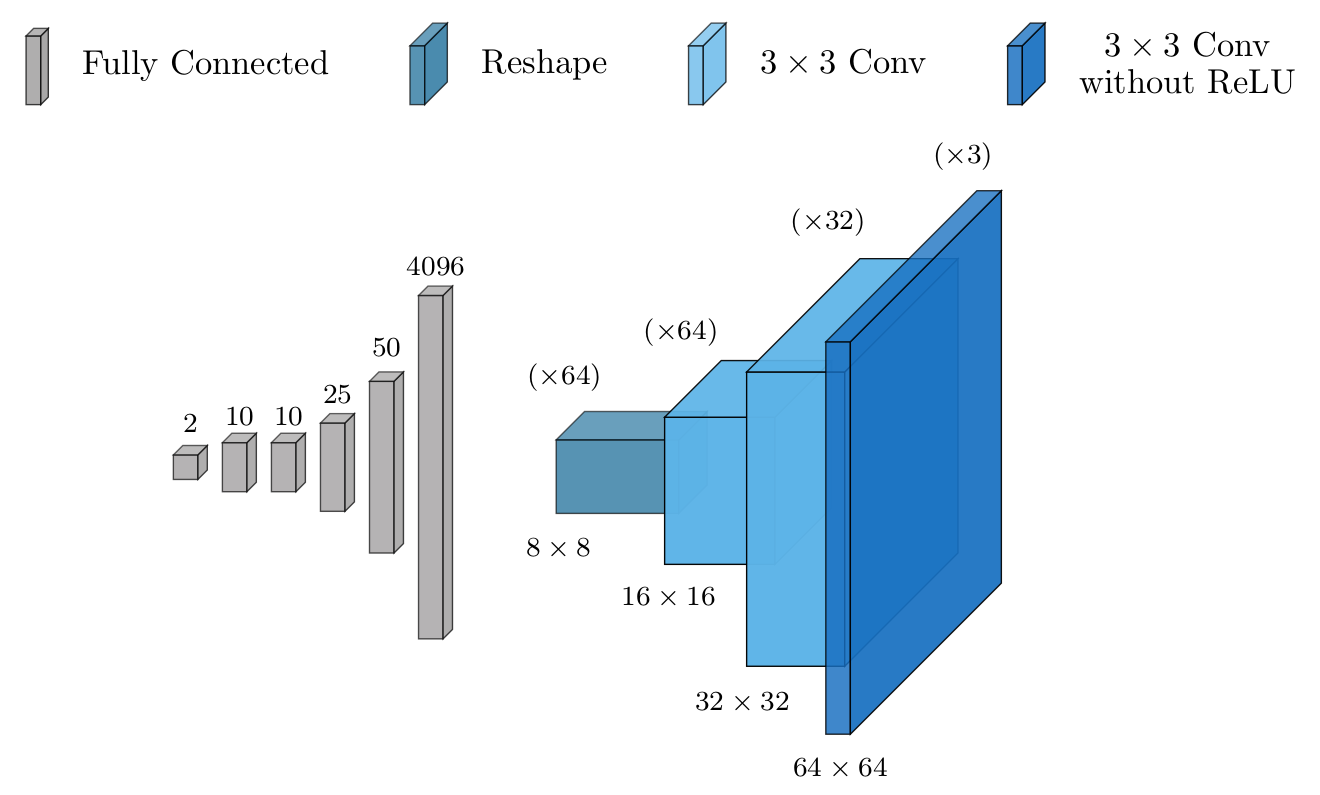
\includegraphics[scale=0.25]{figure/forward_figure.eps}
\caption{Network structure for the forward problem.  Features have been labeled by colors corresponding to the type of network layer used to produce them.}
\label{fig:forward}       
\end{figure}

Of equal importance to the network structure is the choice of a suitable loss function. In order to successfully train the network for the forward problem, it was necessary to design a loss function which converted the raw LAMMPS damage data into a format which is compatible with the deep learning framework and array/tensor-based format of the TensorFlow network implementation.  This conversion was performed most naturally by bucketizing the atoms into a uniform grid of resolution $64 \times 64$.  The average damage of the atoms contained in each bucket/bin of the grid was calculated and used to create the target outputs for the network.  It was also necessary to account for atoms which had been substantially dislocated by a direct impact with the indenter and had left some bins at the disk’s interior empty.  These interior bins were assigned a full damage value of 1.0 to indicate that the atom which had originally occupied the space was displaced by the indenter.  This was achieved by storing a copy of the LAMMPS data before the indenter strikes to serve as a template which indicates where the atom damages should be calculated.
This loss function was defined using the neural network prediction $y^*$, true discretized damage pattern $y$ obtained from the LAMMPS simulation, and template $T$ described in section \ref{forward_data}.
The mean square error (MSE) was then calculated on the interior of the disk using the template file as an indicator of where the interior error should be calculated:

\[
\operatorname{Loss}(y^*, y) \, \, = \, \, \frac{1}{N^2} \, \sum_{i=1}^N \, \sum_{j=1}^N \, \, \mathbbm{1}_{T}[i,j] \cdot \left| \, y^*[i,j] \, - \, y[i,j]  \, \right|^2
\]


%Here we denote the network prediction by $y^*$, the true damage pattern by $y$,
Here $N$ denotes the selected output resolution, and $\mathbbm{1}_T$ denotes the indicator for the Boolean template file $T$  (i.e. $\mathbbm{1}_{T}[i,j]=1$ when the $(i,j)^{th}$ bin was originally occupied by an atom, and $\mathbbm{1}_{T}[i,j]=0$ otherwise).


All network layers used ReLU activation functions except for the final layer; as the damage pattern values are scaled to be within the range between $0$ and $1$, the final network layer was equipped with a sigmoidal activation function:


\[
\operatorname{sigmoid}(x) \, \, = \, \, \frac{1}{1 \, + \, \exp(-x)}
\]

The model was trained using the standard ADAM optimization algorithm and backpropagation as implemented in TensorFlow.  The learning rate for the ADAM optimizer was initialized to 0.0001 with a geometric decay rate of 0.9 applied every 3 epochs.  The model was trained for 100 epochs using 20,200 training data points, with the remaining 5,050 data points reserved for testing/validation.  



\subsubsection{Forward problem results and discussion}
\label{forward_results}

\begin{figure}
  \centering
  %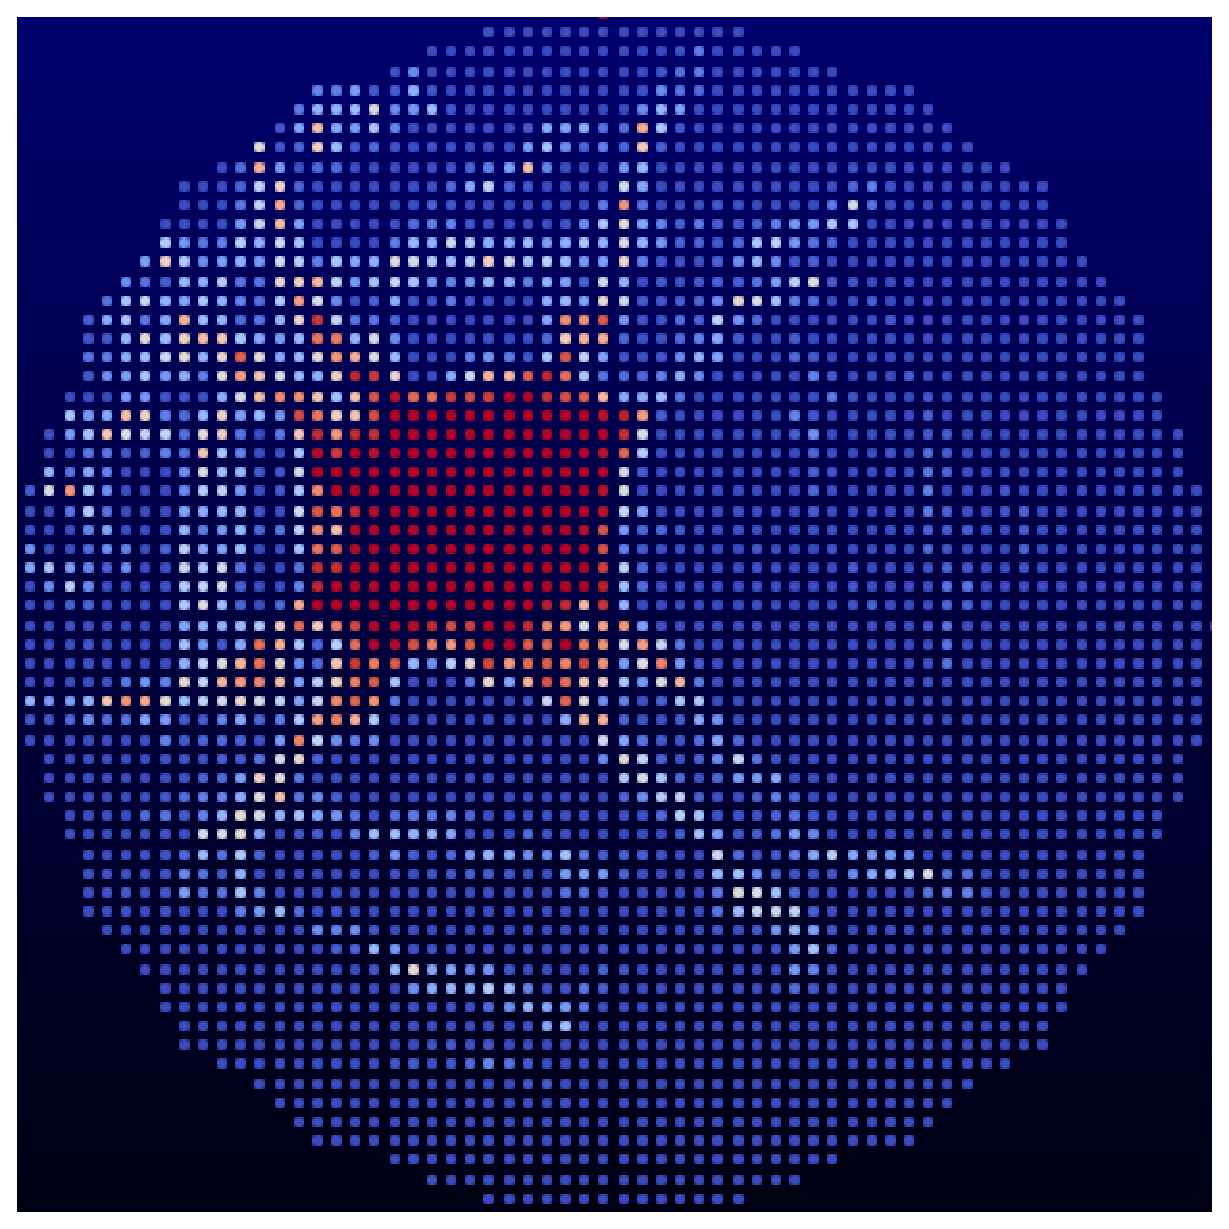
\includegraphics[scale=0.25]{figure/true_soln_2300.eps}
  %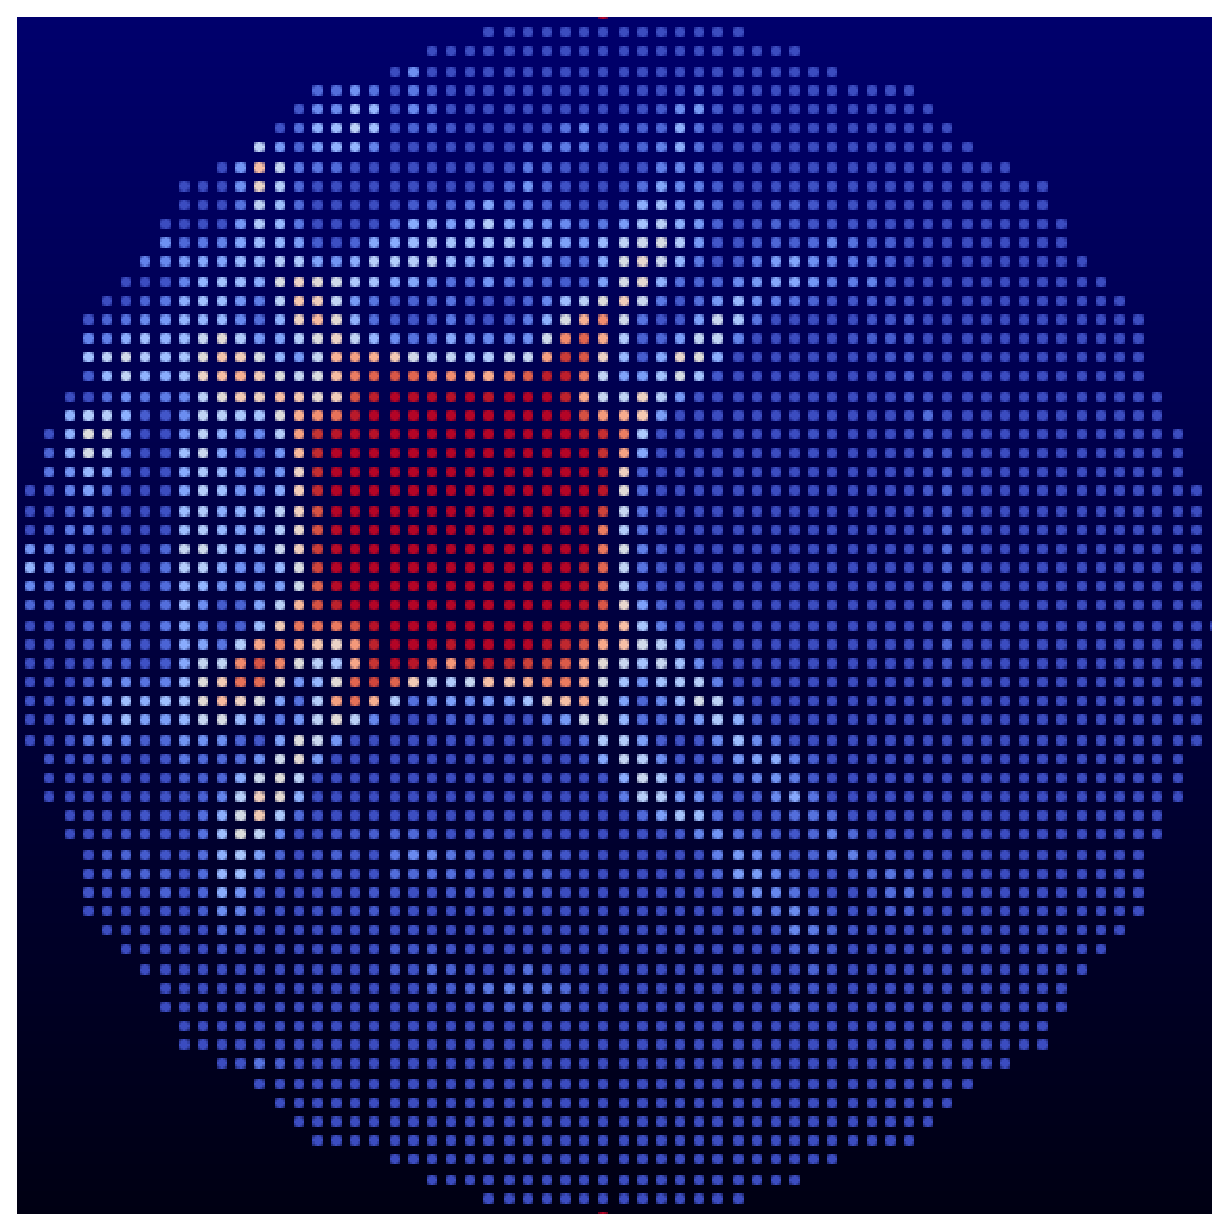
\includegraphics[scale=0.25]{figure/prediction_2300.eps}
  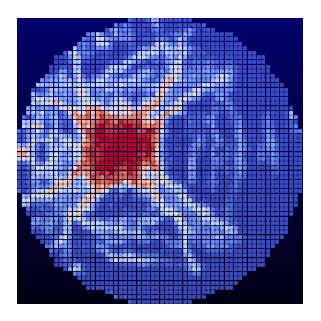
\includegraphics[scale=1.1]{figure/New_Solutions/soln_19050.eps}
  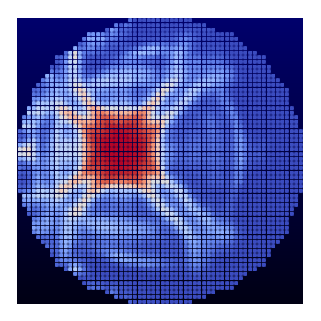
\includegraphics[scale=1.1]{figure/New_Solutions/pred_19050.eps}
\caption{Example of a true damage pattern computed using LAMMPS (left) along with the corresponding neural network prediction (right).}
\label{fig:forward_results}       
\end{figure}


\begin{table}
  \centering
  \begin{tabular}{c|c|c|c}
    Dataset  &  Avg. Computation Time  & Avg. MSE &  Avg. $L^1$ Error \\ \hline
    %Training &    0.002253 s &    0.010207  &   0.054351  \\ 
    %Testing  &    0.002273 s &    0.010316  &   0.054664
    Training &    0.003973 s &    0.010214  &   0.054590  \\ 
    Testing  &    0.003970 s &    0.010298  &   0.054779  
  \end{tabular}
  \caption{Average computation times, MSE, and $L^1$ errors for the forward problem model.}
  \label{fig:forward_results_table}
\end{table}


After training, the neural network's damage predictions are seen to closely approximate the true damage patterns from the LAMMPS simulations.  The offline training procedure required just under 7 hours to complete using 4 CPUs; once completed, network predictions for damage patterns can be computed in less than $0.0025$ seconds with average MSE and $L^1$ errors in the range of $0.01$ and $0.05$, respectively (see Table~\ref{fig:forward_results_table}).  Of note is the fact that a single LAMMPS simulation for the specified problem setup required an average of $6$ seconds to complete on the same machine;  the trained network is thus seen to  provide approximations to the true simulation results while reducing the computation time  by a factor of over $1500$.




\begin{figure}
  \centering
  \begin{tabular}{ccc}
  %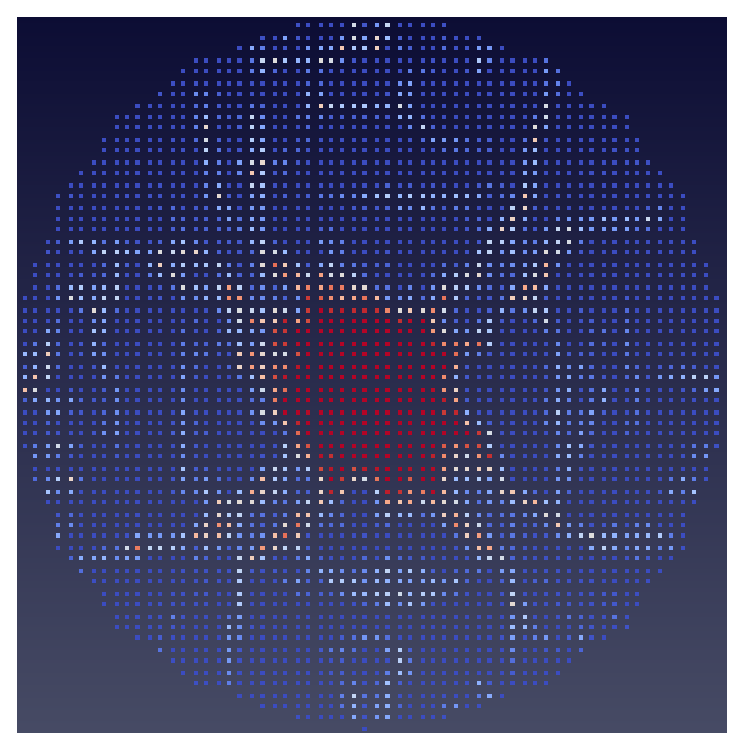
\includegraphics[scale=0.3]{figure/Solutions/solution_200.eps} &
  %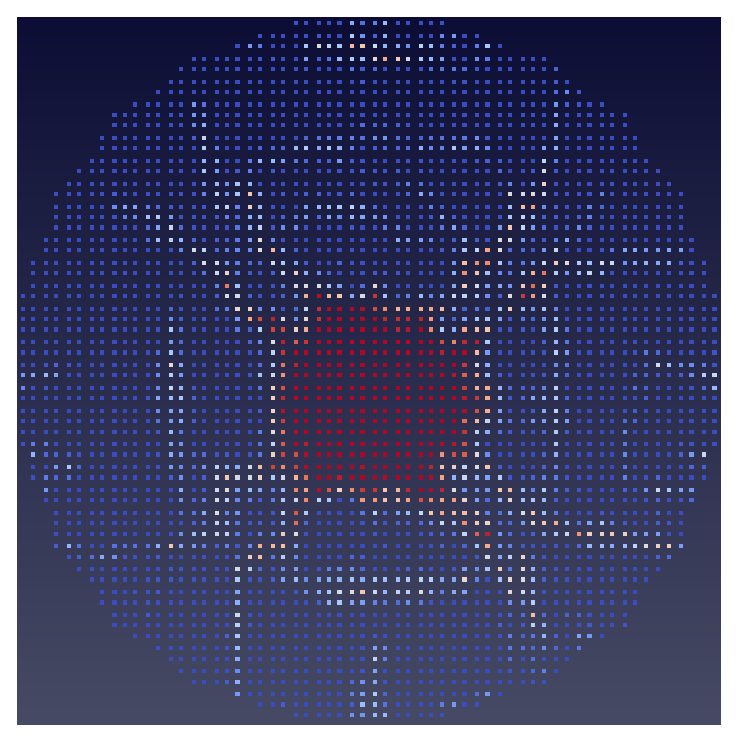
\includegraphics[scale=0.3]{figure/Solutions/solution_201.eps} &
  %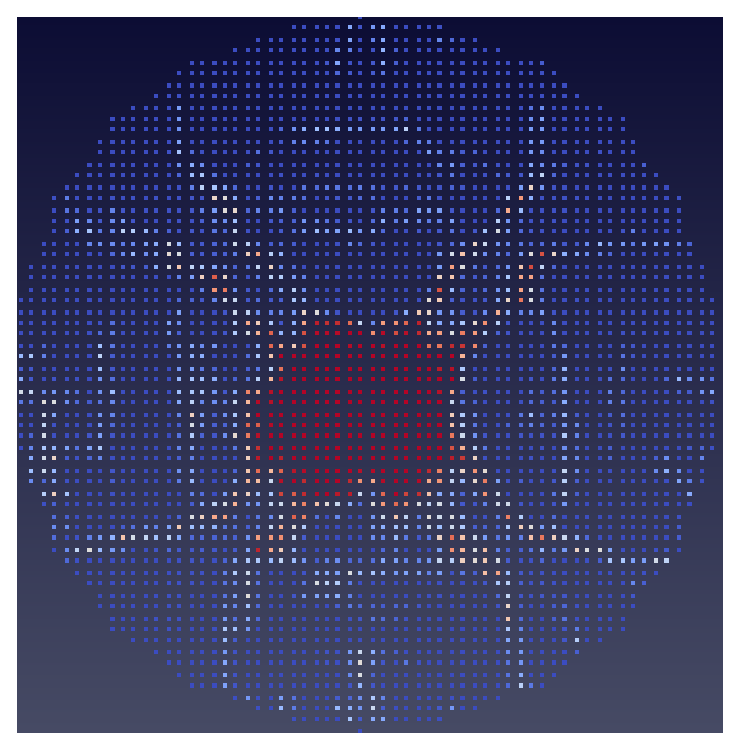
\includegraphics[scale=0.3]{figure/Solutions/solution_202.eps} \\
  %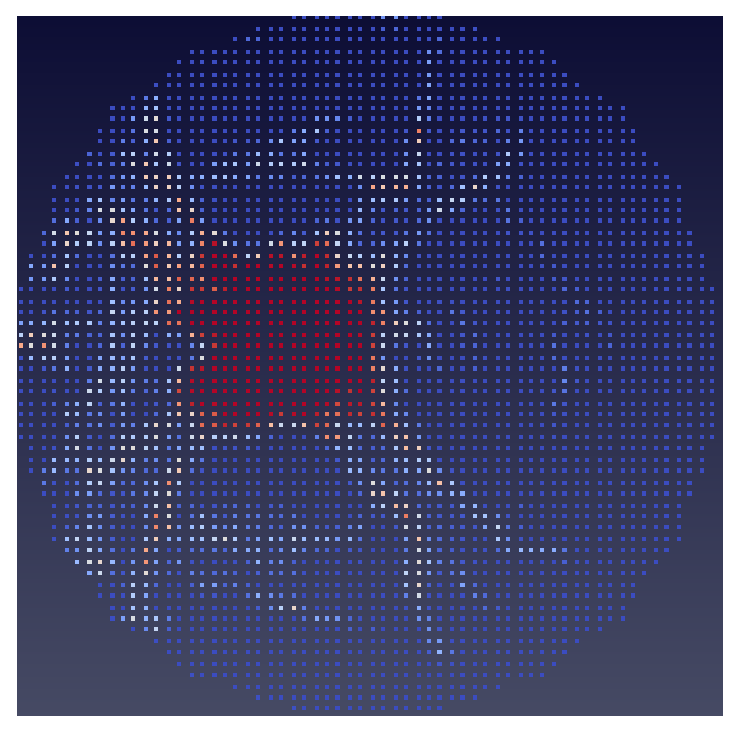
\includegraphics[scale=0.3]{figure/Solutions/solution_2000.eps} &
  %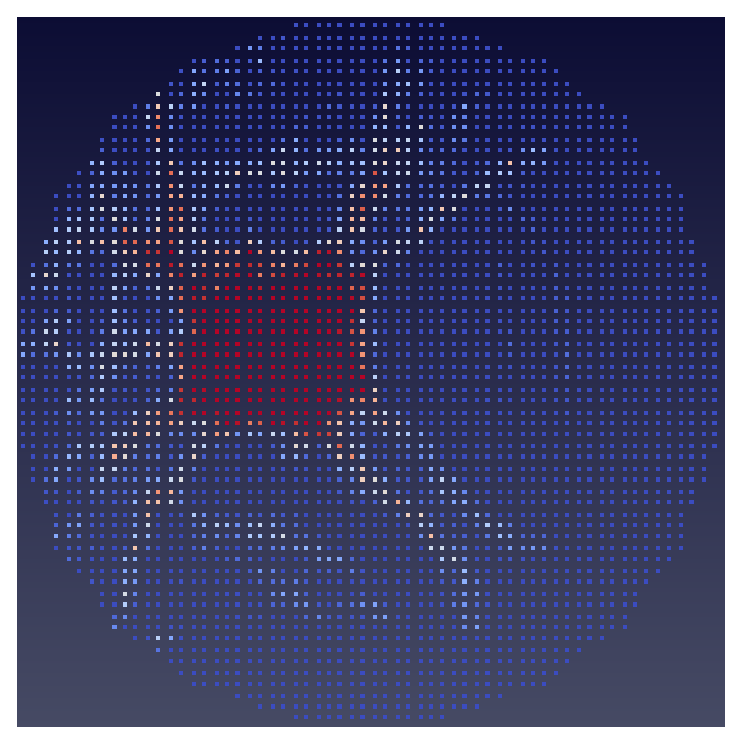
\includegraphics[scale=0.3]{figure/Solutions/solution_2001.eps} &
  %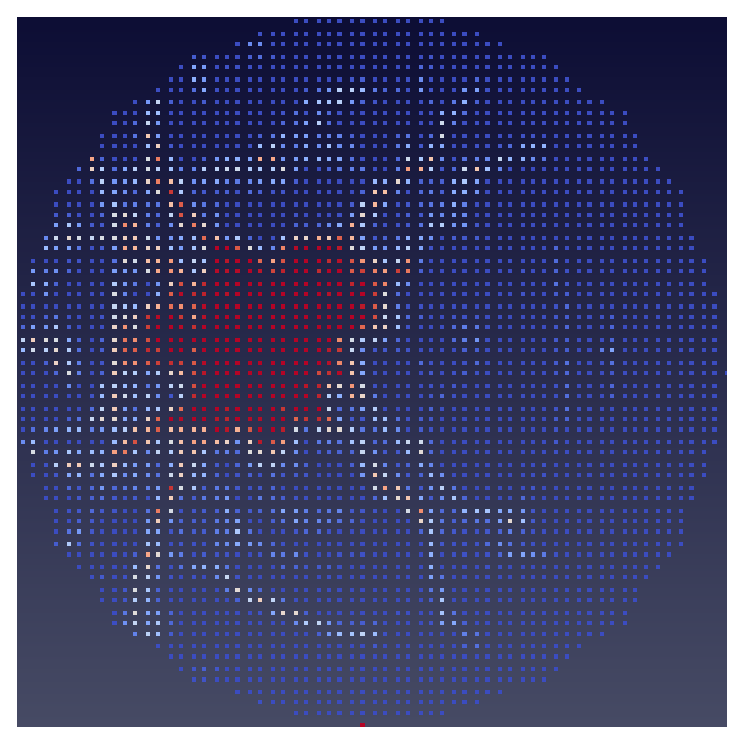
\includegraphics[scale=0.3]{figure/Solutions/solution_2002.eps}
  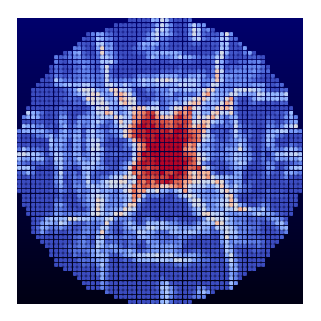
\includegraphics[scale=0.75]{figure/New_Solutions/true_soln_1510.eps} &
  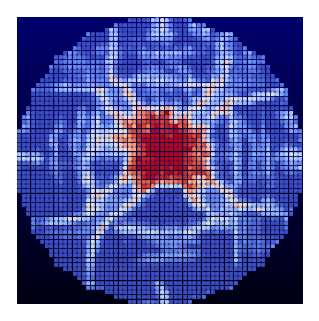
\includegraphics[scale=0.75]{figure/New_Solutions/true_soln_1511.eps} &
  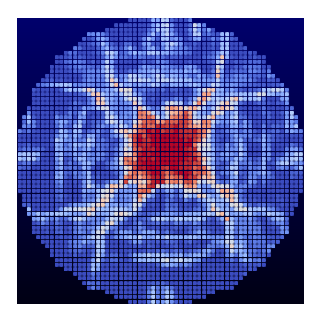
\includegraphics[scale=0.75]{figure/New_Solutions/true_soln_1512.eps} \\
  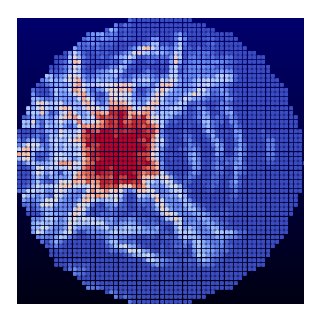
\includegraphics[scale=0.75]{figure/New_Solutions/true_soln_19049.eps} &
  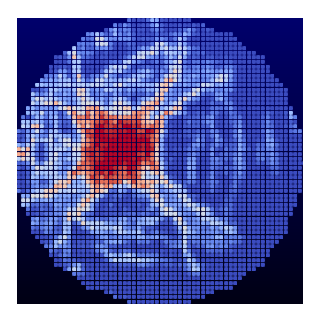
\includegraphics[scale=0.75]{figure/New_Solutions/true_soln_19050.eps} &
  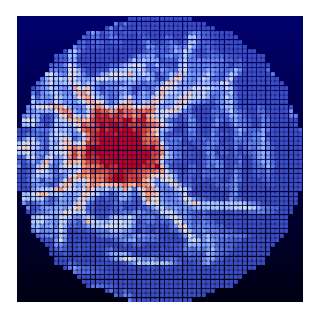
\includegraphics[scale=0.75]{figure/New_Solutions/true_soln_19051.eps} 
  \end{tabular}
  \begin{tabular}{lcclc}
  %Top-Left:   &  (0.001139, -0.003129) & & Bottom-Left:   & (-0.010100, 0.002305) \\
  %Top-Center: &  (0.000692, -0.003257) & & Bottom-Center: & (-0.009987, 0.002756) \\
  %Top-Right:  &  (0.000232, -0.003322) & & Bottom-Right:  & (-0.009853, 0.003201) \\
  Top-Left:   &  (0.001471, 0.002675) & & Bottom-Left:   & (-0.010236, 0.002842) \\
  Top-Center: &  (0.001603, 0.002598) & & Bottom-Center: & (-0.010193, 0.002989) \\
  Top-Right:  &  (0.001732, 0.002514) & & Bottom-Right:  & (-0.010275, 0.002694) \\
  \end{tabular}
\caption{Demonstration of low forward stability of true damage patterns for LAMMPS simulations.  A cluster of neighboring hit locations near the center of the disk (top row) as well as a cluster further from the center (bottom row) both produce a widely varied collection of simulated damage patterns (coordinates of each hit location are shown below the figures).}
\label{fig:forward_solutions}       
\end{figure}


As depicted in Fig.~\ref{fig:forward_results}, we see that the overall pattern of the damage on the disk is predicted quite well, however many of the finer details have been deemphasized or smoothed out by the network.  The network predictions also tend to be more symmetric than the simulated patterns, and tend to produce more linear cracking branches in contrast to the more jagged cracks from the simulations.
%
The reason why the predictions are overly symmetric is most likely due to the relatively low forward stability of the LAMMPS peridynamics simulations.  That is to say that the damage patterns are observed to change significantly even when the hit location of the indenter is changed by a very small amount.  For example, the patterns shown in Fig.~\ref{fig:forward_solutions} correspond to hit locations which are very close to one another near the center of the disk along with a cluster of hit locations further from the center.
%%

Each of these clusters has a maximum distance of less than $0.00031$mm on a disk of radius $0.037$mm (i.e. less than $0.85\%$ of the radius), yet the simulated damage patterns are seen to be quite disparate.  It is suspected that the smoother, more symmetric neural network predictions illustrated in Fig.~\ref{fig:forward_results} may be reflective of the average damage incurred when the indenter's hit location is varied over a small neighborhood of the precise location provided to the network as input.





%\vspace{0.1in}
%\noindent\begin{tabular}{@{}lcclc}
%Top-Left:   &  (0.001139, -0.003129) & & Bottom-Left:   & (-0.010100, 0.002305) \\
%Top-Center: &  (0.000692, -0.003257) & & Bottom-Center: & (-0.009987, 0.002756) \\
%Top-Right:  &  (0.000232, -0.003322) & & Bottom-Right:  & (-0.009853, 0.003201) \\
%\end{tabular}
%\begin{tabular}{lc}
%Bottom-Left:   & (-0.010100, 0.002305) \\
%Bottom-Center: & (-0.009987, 0.002756) \\
%Bottom-Right:  & (-0.009853, 0.003201) \\
%\end{tabular}
%%


%4.1.1
%\subsubsection{Preparation of data}
%\label{subsubsec1}

%4.1.2
%\subsubsection{Reference annotation}
%\label{subsubsec2}

%4.1.3
%\subsubsection{Experiment-specific training and testing}
%\label{subsubsec3}

%4.1.4
%\subsubsection{Prediction accuracy}
%\label{subsubsec4}

%4.2
\subsection{Datasets of the inverse problem}
\label{subsec1}

%The neural network model used for the inverse problem
The inverse problem 
follows a supervised machine learning setup which uses labeled input and output data for training.
%{\rd{Labeled input and output data are required to apply the supervised machine learning algorithm in this experiment.}}
%%
%{\rd{Various types of data are available to be used as input data.}}
%%
%{\rd{Moreover, the features of the input data are determined, and it is usually expressed in vector form.}}
%%
%For the data set, image forms of damage data, which is simulated by LAMMPS, are used as an input data set.
The input data for the inverse problem consists of damage pattern arrays obtained from LAMMPS simulations,
which we will denote by $\mathcal{X}$=\{$\mathcal{X}_1$,$\mathcal{X}_2$,...,$\mathcal{X}_N$\} with  $N\in\mathbb{N}$.
%%
%{\rd{Let the damage data be}} $\mathcal{X}$=\{$\mathcal{X}_1$,$\mathcal{X}_2$,...,$\mathcal{X}_N$\} as an input data when  $N\in\mathbb{N}$.
%%
% For supervised machine learning, labels which classify and represent the input data are required as well.
%%
Each damage pattern $X_i$ is classified by a label $\omega_i \in$ \{$\omega_1$,$\omega_2$,...,$\omega_M$\} which corresponds to the indenter mode (i.e.\! parameter setup) used to create that damage pattern.
 %{\rd{Consider the label set $\omega$=\{$\omega_1$,$\omega_2$,...,$\omega_M$\} in case $M\in\mathbb{N}$, and each label is assigned to the corresponding input data $\mathcal{X}$.}}
%%
The complete labeled data set then consists of the collection of all {\emph{training pairs}} $($\mathcal{X}_i$, $\omega_i$).
%%
%%
 % In this work, 70\% of the input data and 10\% of the input data set are used for the training set and the test set respectively and 30\% of the training data, is used for the validation set.
  In this work, 60\% of the data set examples have been used for training, 25\% of the data is used for validation, and 15\% is used for testing the model.
%%
%%
% The goal of the supervised machine learning algorithm is to efficiently {\rd{classify the training set according to the corresponding labels.}}
%%
 There are a few supervised learning algorithms which are used such as decision trees, Naive Bayes, Artificial Neural Network (ANNs), etc \cite{Ref21}.
%%
 In this paper, Convolutional Neural Networks (CNNs) are used as the supervised learning algorithm.
 %%
 The labeled training and validation sets are used to train the neural network which is designed to approximate the function $\mathcal{F}$: $ \mathcal{X}_i$ $\rightarrow$ $\omega_i$
 which maps the input damage patterns to the indenter mode which has been used to produce them.
 %%
% {\rd{Through the learning algorithm, the labeled training set and validation set are used as an input of a function which allows the learning algorithm to classify the relationship between the unlabeled input data $\mathcal{X}$ and the corresponding labels $\omega$.}}
%%
% Thus, it generates a function $\mathcal{F}$: $ \mathcal{X}_i$ $\rightarrow$ $\omega_i$ designed to map damage patterns to the collection of indenter parameters which result in similar pattern.
%%
 %{\rd{ Moreover, through the validation set which is sorted from the input data, the function is optimized as a classifier, and it makes an accurate prediction model.}}
 The validation set is used to identify and eliminate overfitting in the model and is also used to tune model hyperparameters.
 %%

 
 In order to evaluate the prediction model, a separate set of data, referred to as the test set, is used to assess the accuracy of the model.
%%
%{\rd{ In the same way as the training set, the corresponding labels is assigned to the new test set.}}
%%
%{\rd{ This test set is sent to the prediction model, and it finally shows the accuracy of the prediction model by predicting the assigned labels of the test set.}}
%%
%In this process, the labels of the test set are not used for training but for prediction.
Since the data from the test set is never used during training, the accuracy of the model predictions on this set provides a measure of how well the model generalizes beyond the data that it has already seen.
%%
 Thus, the prediction model predicts the corresponding labels of each component of the data set, and the predicted labels are compared with the desired labels of the test pairs.
%%
 The success rate of prediction on the test set is used as the primary evaluation measure, and it shows the accuracy of the model achieved by the learning procedure. %supervised learning algorithm.
 %%


In this section we introduce a neural network model designed to approach the {\emph{inverse problem}} associated with the peridynamics crack simulations.
%%
%%
In general, solving an inverse problem entails recovering the initial conditions of a simulation from the final result.
%%
More specifically, the inverse problem considered in this section consists of recovering the specific mode of indenter parameters which have been used to produced a specified crack pattern.
%%
To this end, a CNN model is introduced which is designed to predict the velocity, radius, and impact angle corresponding to a given input crack pattern.
%An inverse problem is a mathematical way to predict the parameters through the measured and observed data.
%%
%In this work, the crack pattern on a disk by an indenter was supposed to be analyzed depending on the different value of the parameters of the indenter through the way of the inverse problem.
%%
%{\rd{ The purpose of this section is using the concept of the inverse problem for the crack pattern to predict the velocity, radius, angle and hitting points of the indenter.}}

%4.2.1
\subsubsection{Preparation of data}
\label{subsubsec1}
%table1
\begin{table}[h!]
\centering
\caption{Setup for 8mode of input image data.}
\label{tab:1}       
\begin{tabular}{c|c}
\hline
\hline
Mode & 4variables \\
\hline
 & Radius of indenter (r) = 0.007, 0.008m \\
 & Velocity of indenter (v) = 100, 100.1m/s \\
 & Angle of indenter (a) = 0$^{\circ}$ ,45$^{\circ}$  \\
 & Hitting location of disk (x, y) \\
 \hline
Mode1 & r=0.007m, v=100m/s, 0$^{\circ}$ \\
Mode2 & r=0.007m, v=100.1m/s, 0$^{\circ}$ \\
Mode3 & r=0.008m, v=100m/s, 0$^{\circ}$ \\
Mode4 & r=0.008m, v=100.1m/s, 0$^{\circ}$ \\
Mode5 & r=0.007m, v=100m/s, 45$^{\circ}$ \\
Mode6 & r=0.007m, v=100.1m/s, 45$^{\circ}$ \\
Mode7 & r=0.008m, v=100m/s, 45$^{\circ}$ \\
Mode8 & r=0.008m, v=100.1m/s, 45$^{\circ}$ \\
\hline
\end{tabular}
\end{table}
%Matconvnet \cite{Ref22} based on MATLAB code was applied to the inverse problem using numpy array as input image data.
The MATLAB toolbox Matconvnet~\cite{Ref22} has been applied to the inverse problem using damage pattern arrays of resolution $128\times128$ as input data.
%%
%{\rd{ Prior to considering the results,}} focusing on the input data using LAMMPS, {\rd{
The output data, corresponding to the classification of indenter parameters, can be classified into 8 modes;
these modes correspond to the values of the radius, velocity, and impact angle of the indenter as shown in Table 2.
%%
The hitting location on the disk has also been varied to create a data set with 5,040 training examples, 2,160 validation examples, and 1,200 test examples.
%%


%%
% The mode according to the variation of the variable is set as a combination of the velocity, angle, radius of the indenter and the hitting location of the disk and is shown in Table. 2.
%%
% Training data set and test data set are distinguished to apply input image data set to machine learning algorithm.
%%
% The array size of the inputs has been selected to be 128 pixels by 128 pixels. % and the number is 7200.
%%
% 2,160 (30\% of 7,200 training data set) were designated as a validation set.
% {\rd{[The validation set is supposed to be separate from the training set; is this the case?]}}
%%
% {\rd{In this way, the image size of the test data set is 128 pixels by 128 pixels, and the number of images is 1200.}}
%%
% {\rd{360 (30\% of 1,200 test data set) were designated as a validation set in the test data set.}}
%4.2.2

\subsubsection{Reference annotation}
\label{subsubsec2}

\begin{figure}
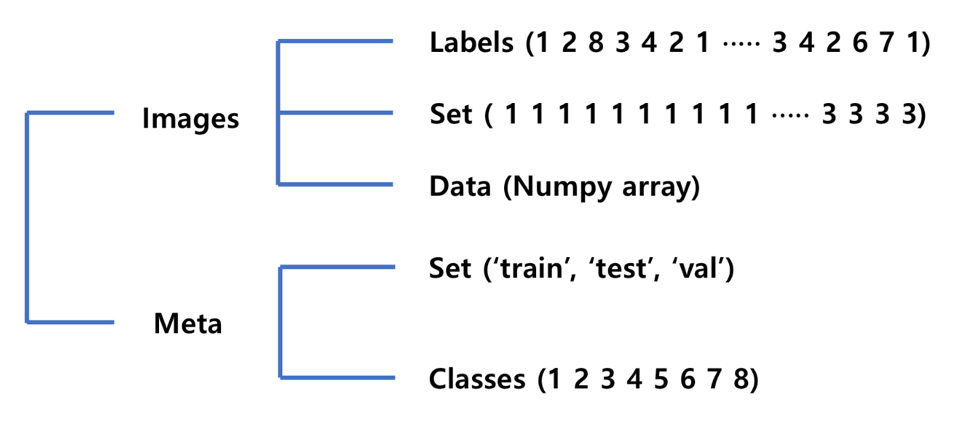
\includegraphics[width=10cm, height=5cm]{figure/label.eps}
\caption{Structure of data in the .mat file}
\label{fig:4}       
\end{figure}
The training data set and the test data set are made into a .mat file that can be applied to Matconvnet and its structure is shown in Fig. 7. The structure of the data in the .mat file is largely divided into `Images' and `Meta'. There are `Labels', `Set' and `Data' classes in the `Images' class. `Labels' displays labels on images of input data sets. Labels were displayed randomly from 1 to 8 since data has 8modes. In the set class, training data, test data, and validation data are indicated by 1, 2, and 3, respectively. In the `Data' class, the data obtained from the LAMMPS is converted to a numpy array and expresses it as a 4-D single matrix. Finally, there are `Set' and `Classes' in the `Meta' class. The `Set' contains the words `train', `test' and `val' which are related to the `Images' class and indicate that the 1 2 3 in the set of images class is training data, test data and validation data respectively. The `Classes' in the `Meta' specifies a class from 1 to 8 due to this inverse problem has a mode of 8.
\begin{figure}
\includegraphics[width=12cm,height=5cm]{figure/cnn.eps}
\caption{Architecture of convolution neural networks (CNNs) for inverse problem and rectification (ReLU) and downsampling layers (MaxPooling) represented in section 4.1.4. This figure shows the data size, kernel size and the numbers of the output feature and produced by each filter layers.}
\label{fig:5}       
\end{figure}
%4.2.3
\subsubsection{Convolutional neural network for inverse problem}
\label{subsubsec3}
Deep learning is a subset of AI and machine learning capable of achieving state-of-the-art results on problems such as object detection, text generation, and image recognition.
%%
Using existing human knowledge in the form of annotated data, various cognitive and inferential tasks can be performed \cite{Ref23,Ref24,Ref25}.
%%
Convolutional neural networks are widely used to solve computer vision problems such as classification of images and object detection.
%%
These convolutional neural networks consist of several layers which can be tuned through the connection weights between input and output layers.
%%
In this work for damage analysis using machine learning, a similar structure of AlexNet are chosen \cite{Ref26}.
%%
The CNN processes the input damage pattern in two steps: a feature extraction step carried out by the convolutional layers, followed by a classification step performed by the fully connected layers.
%{\rd{The CNNs adjusts two steps through the neural layers such as feature extraction and feature classification.}}
%%
First, feature extraction uses a 2D damage array of size $N_{row}$ $\times$ $N_{col}$ for input data and produces a vector of size 8 $\times$ 8 $\times$ 100.
%%
Second, the feature vector is converted to a classification vector of size 1 $\times$ $N_{c}$, where $N_{c}$ is the number of classification categories.
%%
This work accounts for eight categories corresponding to each of the eight distinct indenter modes.

%4.2.3
\subsubsection{Feature extraction and classification}
\label{subsubsec3}
The purpose of image extraction and classification is to create a 1 $\times$ $f_c$ feature vector in relation to the input data, which is related to the 8 modes used for classification.
%%
The feature vector is generated from the input training data by applying successive filters and the filters are 1) Maxpooling layer, 2) ReLU layer and 3) SoftMax layer; each of the three types of network layers are described below.
\\
\\
1) Maxpooling layer \cite{Ref27} is a sample-based discretization process. The objective is that  downsamples the input images and reduce its size, the computational load, and the memory usage. If the input image $x$ is a square image of size $N_{col}$ $\times$ $N_{row}$, and $a = 2$, then the output image y of the pooling operation is of size [$N_{col}$/a] $\times$ [$N_{row}$/a]. In our research, the downsampling rate is set to $a = 2$,
the 64 pixels by 64 pixels array becomes 32 pixels by 32 pixels and 16 pixels by 16 pixels image becomes 8 pixels by 8 pixels.
\\
\\
2) The rectified linear unit (ReLU) layer \cite{Ref28} applies an activation function which is defined as the positive part of its argument: %and this activation function is shown in Eq.(11).
%%
\begin{equation}
ReLU(x) = x^{+} = \max(0,x) 
\end{equation}
%%
where $x$ is the input data to a neuron. A ReLU performs a threshold operation
to each element of the input where any value less than zero is set to zero.
%%ReLU improves neural network by speeding up training due to the simplicity of evaluating the ReLU activation.
%%
%%The rectified linear unit (ReLU) has been selected as the network's activation function;
The choice of the ReLU activation facilitates faster training due to the simplicity of its function and derivative evaluations.
\\
\\
3) SoftMax layer \cite{Ref29} is often used in the final layer of a neural network-based classifier.  It takes a vector of arbitrary real-valued scores (in z) and reduces it to a vector of values between zero and one that sum to one.

\begin{equation}
z^{[L]}=W^{[L]}a^{[L-1]}+b^{[L]} 
\end{equation}
To compute z, SoftMax activation function is needed.
\begin{equation}
t = \exp z^{[L]}
\end{equation}
t and $z^{[L]}$ is (8,1) dimensional vector which is related to the 8 modes of output.

\begin{equation}
a^{[L]} = \frac{\exp z^{[L]}}{\sum_{i=1}^{8} t_i} 
\end{equation}
output a is going to be the vector t but normalized to sum to 1.



%4.2.4
\subsubsection{Training and testing using CNNs and prediction accuracy}
\label{subsubsec3}

The model for the inverse problem has been trained using the MATLAB toolbox Matconvnet.
%Data was trained by Matconvnet based on MATLAB.
%%
The prediction model has been implemented as a convolution neural network (CNN) with architecture as shown in Fig 8.
%%
The proposed convolutional network is composed of two convolutional layers and a fully-connected layer.
%%
Each convolutional layer is followed by a max pooling layer and rectified linear unit layer (ReLU).
%%
After the two convolution layers, a fully-connected layer with softmax activation is used in the final layer of convolution neural network-based classifier.
%%
In the first convolutional layer, the “weights” are the filters being learned and initialized with random numbers from a Gaussian distribution.
%%
The filters are 2 by 2 spatial resolution with 1 filter depth and the number of kernels is 200.
%%
The next layer is a max pooling layer which takes 2 by 2 sliding window with a stride of 2.
%%
The spatial resolution will be decreased due to the stride 2 in max pooling layer.
%%
%The next layer is the rectified linear unit (ReLU).
The ReLU activation function is then applied to introduce non-linearities into the modeling framework.
%%
%The rectified linear unit (ReLU) has been selected as the network's activation function; this choice facilitates faster training due to the simplicity of evaluating the ReLU function and its derivative.
%%
%{\rd{It promotes the convergence of stochastic gradient descent through the negative value becomes zero.}}
%%
%{\rd{By doing this activation, the enhancement of the speed of convergence can be seen when training the data. }}
\label{subsubsec3}
\begin{figure}
\centering
\includegraphics[height=10cm]{figure/error1.eps}
\caption{Objective and error plots during the training.}
\label{fig:5}       
\end{figure}
The last layer is a fully-connected layer which has dense connections with the activation function outputs from the previous convolution layers.
%%
The final layer is designed to produce 8 ouput values corresponding to the model's predicted likelihood for each of the 8 indenter modes.
%be 1x1 spatial resolution and since the size of the filter should be classified as 8 modes, it should be unconditionally 8.
%%%
Using the CNNs mentioned above with the 7200 training data and the 1200 test data, the learning rate is 0.001, the batch size is 20, and the epoch is 25 for the training. 
%During the training procedure for the CNN, {\rd{each successful epoch produces up to the plots (objective and error plots).}}
%%
In this convolutional neural network, MatConvNet minimizes the objective which represents the loss function and y axis of energy represents to measure the magnitude of loss.
%%
During the training, several statistics are measured after every batch.
%%
In the objective and the error plots, the training error is depicted by the blue line and the validation error is represented by an orange dotted line. The error graph should show similarity to the objective graph and our network achieved 0.044 validation error. Lastly, the results are shown in Table. 3. The left side shows the number of the 10 test images and the marked label among 1200 test images, and the right side shows the prediction based on the training results.
\begin{table}[h!]
\centering
\caption{CNNs predictions results compared to the test image data.}
\label{tab:1}       
\begin{tabular}{c|c}
\hline
\hline
Test image number : Label(Mode) & CNNs prediction results (Mode) \\
\hline
Test image 1 : 5 (Mode) & 5 (Mode) \\
Test image 2 : 6 (Mode) & 6 (Mode) \\
Test image 3 : 7 (Mode) & 7 (Mode) \\
Test image 4 : 2 (Mode) & 2 (Mode) \\
Test image 5 : 8 (Mode) & 8 (Mode) \\
Test image 6 : 7 (Mode) & 7 (Mode) \\
Test image 7 : 2 (Mode) & 1 (Mode) \\
Test image 8 : 3 (Mode) & 3 (Mode) \\
Test image 9 : 8 (Mode) & 8 (Mode) \\
Test image 10 : 6 (Mode) & 6 (Mode) \\
\hline
\end{tabular}
\end{table}
As we can see in Table. 3, labeled test images and CNNs prediction results are quite match the results each other. To evaluate the accuracy of training data obtained from CNNs, the success rate is defined as
\begin{equation} 
%\label{eqn3}
\frac{number\ of\ correct\ test\ images}{total\ number\ of\ test\ images} \times 100\%
\end{equation}
The prediction results of the inverse problem using the training data showed a success rate of 95.6\%.
%5
\section{Conclusion}
\label{sec:5}


We have used the peridynamic-based MD simulation to change the hit locations of the disk, impacting the disk and forming a distinct crack pattern. Based on the crack pattern data obtained from MD simulation, both the forward problem and inverse problem were approximated by convolutional neural networks.  The results for the forward problem were shown to provide accurately predicted damage patterns both quantitatively and qualitatively.  Though the patterns predicted by the network tend to be more symmetric and smooth in comparison with the MD simulation results, it has been seen that this is likely a reflection of low forward-stability in the fine details of the crack patterns for the forward problem.  Although the predictions omit some small-scale features in the crack patterns, the overall structure of the cracks is shown to be predicted accurately and in a fraction of the time required by direct MD simulations (with network predictions computed over $1,500$ times faster).

For the inverse problem, we used the data of the crack pattern obtained by changing the radius, velocity, angle of the indenter, and the hitting position of the disk. In order to predict the mode, we labeled the data and predict the data by CNNs and accurately predict the most cases from MODE1 to MODE8. By implementing CNNs on the inverse problem, we have shown the ability to identify the MODE through the process of learning via CNNs that extracts related functions from the input images by way of the convolution layer, maxpooling layer, and ReLU layer in the feature extraction. Using these functions, data could be divided into MODE1 to MODE8 through the fully connected layer. The reliability of the classification can be ascertained from the class probability vector generated by the softmax layer existing in the feature classification. 

With regard to the forward problem, future work will be directed toward identifying the causes of the noisy simulation data and apparent low forward-stability observed in the dataset.  Experiments simulating differing material properties, e.g. using other pair-styles in LAMMPS, will also be of interest to assess the overall generality of the proposed neural network training procedure.  In addition, we are very interested in extending our work to simulations of higher complexity (e.g. to a simulation which requires hours to conduct) to test the limits of the representational/modeling potential of the convolutional networks used in this work.

%%
For the inverse problem, we will have to do more complex crack pattern studies by applying more variables to the MD simulation data by Peridigm \cite{Ref30}. For instance, in addition to impacting multiple indenters on a disk, it is necessary to study the shape of the crack pattern by varying the thickness or material of the impacted object or the interaction between the cracks generated by the multiple indenters. Also, since the accuracy of the CNNs classification greatly depends on the quality and resolution of the labeled train data for training the networks, it will improve the accuracy of CNNs classification by improving the size change or resolution of the data. 


\section{Data and Code}
\label{sec:6}
The visualization tool can be downloaded from https://www.paraview.org.
The LAMMPS and Tensorflow code for the forward problem are available on the GitHub repository  https://github.com/nw2190/LAMMPS.
The LAMMPS and MatConvNet code for the inverse problem are also available for download at  https://github.com/moonseopkim/inverseproblem.


%6
%\section{Data and Code}
%\label{sec:6}

% For one-column wide figures use
%\begin{figure}
% Use the relevant command to insert your figure file.
% For example, with the graphicx package use
%  \includegraphics{example.eps}
% figure caption is below the figure
%\caption{Please write your figure caption here}
%\label{fig:1}       % Give a unique label
%\end{figure}
%
% For two-column wide figures use
%\begin{figure*}
% Use the relevant command to insert your figure file.
% For example, with the graphicx package use
%  \includegraphics[width=0.75\textwidth]{example.eps}
% figure caption is below the figure
%\caption{Please write your figure caption here}
%\label{fig:2}       % Give a unique label
%\end{figure*}
%

% For tables use
%\begin{table}
% table caption is above the table
%\caption{Please write your table caption here}
%\label{tab:1}       % Give a unique label
% For LaTeX tables use
%\begin{tabular}{lll}
%\hline\noalign{\smallskip}
%first & second & third  \\
%\noalign{\smallskip}\hline\noalign{\smallskip}
%number & number & number \\
%number & number & number \\
%\noalign{\smallskip}\hline
%\end{tabular}
%\end{table}


\begin{acknowledgements}
We gratefully acknowledge the support from National Science foundation (DMS-1555072, DMS-1736364 and DMS-1821233).
\end{acknowledgements}



%\usepackage{biblatex}
% BibTeX users please use one of
%\bibliographystyle{spbasic}      % basic style, author-year citations
%\bibliographystyle{spmpsci}      % mathematics and physical sciences
%\bibliographystyle{spphys}       % APS-like style for physics
%\bibliography{sample}   % name your BibTeX data base

% Non-BibTeX users please use
\begin{thebibliography}{}
%
% and use \bibitem to create references. Consult the Instructions
% for authors for reference list style.
%
% Format for Journal Reference
%Author, Article title, Journal, Volume, page numbers (year)
% Format for books
%\bibitem{Ref2}
%Author, Book title, page numbers. Publisher, place (year)

\bibitem{Ref1}
Seleson, P., Parks, M. L., Gunzburger, M., \& Lehoucq, R. B. (2009). Peridynamics as an upscaling of molecular dynamics. Multiscale Modeling \& Simulation, 8(1), 204-227.

\bibitem{Ref2}
Silling, S., Epton, A., Weckner, M., Xu, O., \& Askari, J. (2007). Peridynamic States and Constitutive Modeling. Journal of Elasticity, 88(2), 151-184.

\bibitem{Ref3}
Silling, S. (2000). Reformulation of elasticity theory for discontinuities and long-range forces. Journal of the Mechanics and Physics of Solids, 48(1), 175-209.

\bibitem{Ref4}
Silling, S., \& Askari, E. (2005). A meshfree method based on the peridynamic model of solid mechanics. Proposed for Publication in Computers and Structures., 83(17-18), Proposed for publication in Computers and Structures., 2005, Vol.83(17-18).

\bibitem{Ref5}
Bobaru, F., Silling, S. A., \& Jiang, H. (2005). Peridynamic fracture and damage modeling of membranes and nanofiber networks. In XI Int. Conf. Fract., Turin, Italy.

\bibitem{Ref6}
Askari, E., Xu, J., \& Silling, S. (2006). Peridynamic analysis of damage and failure in composites. In 44th AIAA aerospace sciences meeting and exhibit (p. 88).

\bibitem{Ref7}
Kilic, B., Madenci, E., \& Ambur, D. (2006). Analysis of brazed single-lap joints using the peridynamics theory. In 47th AIAA/ASME/ASCE/AHS/ASC Structures, Structural Dynamics, and Materials Conference 14th AIAA/ASME/AHS Adaptive Structures Conference 7th (p. 2267).

\bibitem{Ref8}
Oterkus, \& Madenci. (2017). Peridynamic modeling of fuel pellet cracking. Engineering Fracture Mechanics, 176, 23-37.

\bibitem{Ref9}
Taylor, Michael. (2016). Peridynamic Modeling of Ruptures in Biomembranes. PLoS ONE,11(11), 1-15.

\bibitem{Ref10}
Nikabdullah, N., Azizi, Alebrahim, Singh, and K. "The Application of Peridynamic Method on Prediction of Viscoelastic Materials Behaviour." AIP Conference Proceedings 1602.1 (2014): 357-63. Web.

\bibitem{Ref11}
Prakash, Naveen. (2016). Electromechanical peridynamics modeling of piezoresistive response of carbon nanotube nanocomposites. Computational Materials Science, 113, 154-171.

\bibitem{Ref12}
Platt, P. (2017). Peridynamic simulations of the tetragonal to monoclinic phase transformation in zirconium dioxide. Computational Materials Science, 140, 322-334.

\bibitem{Ref13}
Lall, P., Shantaram, S., \& Panchagade, D. (2010). Peridynamic-models using finite elements for shock and vibration reliability of leadfree electronics. Thermal and Thermomechanical Phenomena in Electronic Systems (ITherm), 2010 12th IEEE Intersociety Conference on, 1-12.

\bibitem{Ref14}
Ahadi, Hansson, \& Melin. (2016). Indentation of thin copper film using molecular dynamics and peridynamics. Procedia Structural Integrity, 2, 1343-1350.

\bibitem{Ref15}
Parks, M. L. (2016). Nonlocal Models and Peridynamics (No. SAND2016-0673PE). Sandia National Lab.(SNL-NM), Albuquerque, NM (United States).

\bibitem{Ref16}
Plimpton, S. (1995). Fast Parallel Algorithms for Short-Range Molecular Dynamics. Journal of Computational Physics, 117(1), 1-19.

\bibitem{Ref17}
Parks, M. L. (2016). Nonlocal Models and Peridynamics (No. SAND2016-0673PE). Sandia National Lab.(SNL-NM), Albuquerque, NM (United States).

\bibitem{Ref18}
Parks, M. L., Seleson, P., Plimpton, S. J., Silling, S. A., \& Lehoucq, R. B. (2011). Peridynamics with lammps: A user guide, v0. 3 beta. Sandia Report (2011–8253).

\bibitem{Ref19}
S. J. Plimpton, Pizza.py http://www.cs.sandia.gov/~sjplimp/pizza.html.

\bibitem{Ref20}
Kitware Inc., ParaView web page. http://www.paraview.org/.


\bibitem{Ref21}
S. Kotsiantis, “Supervised learning: A review of classification techniques,” Informatica, vol. 31, pp. 249–268, 2007.

\bibitem{Ref22}
Vedaldi, Andrea, and Karel Lenc. "MatConvNet - Convolutional Neural Networks for MATLAB." (2014). Web.

\bibitem{Ref23}
Goodfellow, I., Bengio, Y., Courville, A., \& Bengio, Y. (2016). Deep learning (Vol. 1). Cambridge: MIT press.

\bibitem{Ref24}
Géron, A. (2017). Hands-on machine learning with Scikit-Learn and TensorFlow: concepts, tools, and techniques to build intelligent systems. " O'Reilly Media, Inc.".
\bibitem{Ref25}
LeCun, Y., Bengio, Y., \& Hinton, G. (2015). Deep learning. nature, 521(7553), 436.
\bibitem{Ref26}
Krizhevsky, A., Sutskever, I., \& Hinton, G. E. (2012). Imagenet classification with deep convolutional neural networks. In Advances in neural information processing systems (pp. 1097-1105).
\bibitem{Ref27}
Riesenhuber, M., \& Poggio, T. (1999). Hierarchical models of object recognition in cortex. Nature neuroscience, 2(11), 1019.
\bibitem{Ref28}
Krizhevsky, A., Sutskever, I., \& Hinton, G. E. (2012). Imagenet classification with deep convolutional neural networks. In Advances in neural information processing systems (pp. 1097-1105).
\bibitem{Ref29}
Nasrabadi, N. M. (2007). Pattern recognition and machine learning. Journal of electronic imaging, 16(4), 049901.

\bibitem{Ref30}
Parks, M. L., Littlewood, D. J., Mitchell, J. A., \& Silling, S. A. (2012). Peridigm Users’ Guide v1. 0.0. SAND Report, 7800.

\end{thebibliography}

\end{document}



% LocalWords:  peridynamics Moonseop Guang Wontae Jeong indenter ANNs
% LocalWords:  nonlocal Convolutional thermoelectric multiscale piezo
% LocalWords:  nanofiber biomembranes viscoelastic nanocomposites PMB
% LocalWords:  convolutional CNNs LAMMPS peridynamic Microelastic pmb
% LocalWords:  peri Paraview LAMPPS bucketizing upsampled discretized
% LocalWords:  MSE th backpropogation CPUs Matconvnet numpy ReLU
% LocalWords:  downsampling MaxPooling AlexNet Maxpooling SoftMax
% LocalWords:  discretization dimensionality
